\documentclass[12pt]{article}

% Packages for enhanced typesetting and functionality
\usepackage{amsmath, amssymb, amsthm}      % Math symbols and environments
\usepackage{graphicx}                      % For including images
\usepackage{fancyhdr}                      % For header and footer customisation
\usepackage{geometry}                      % For margin customisation
\usepackage[colorlinks=true, linkcolor=blue, urlcolor=blue, citecolor=blue]{hyperref} % Clickable links
\usepackage{xcolor}                        % For coloured text
\usepackage{tikz}                          % For drawing diagrams and flowcharts
\usepackage{algorithm}                     % For algorithms
\usepackage[noend]{algpseudocode}          % For algorithm pseudocode

% Page layout settings
\geometry{margin=1in}
\setlength{\parindent}{0pt}
\setlength{\parskip}{1ex}

% Header and footer
\pagestyle{fancy}
\fancyhf{}
\setlength{\headheight}{15pt}
\fancyhead[L]{Solving Air Crew Scheduling Problems}
\fancyhead[R]{Max Hart}
\fancyfoot[C]{\thepage}

\begin{document}

% Title Page
\begin{titlepage}
    \centering
    \vspace*{1cm}
    
    % University logo (adjust image file as needed)
    
\includegraphics[width=0.4\textwidth]{UoB.jpg}\par\vspace{1cm}
    
    {\LARGE\bfseries Solving Air Crew Scheduling Problems\par}
    \vspace{0.5cm}
    {\Large A Simulated Annealing and Genetic Algorithm Approach\par}
    \vspace{0.75cm}
    
    {\large Evolutionary Computation\par}
    \vspace{1.5cm}
    
    {\large\textbf{Author:} Max Hart\par}
    \vspace{0.3cm}
    {\normalsize \href{mailto:mah422@student.bham.ac.uk}{mah422@student.bham.ac.uk}\par}
    \vspace{1.5cm}
    
    {\large\textbf{Professors:} Dr Shan He and Dr Per Kristian Lehre\par}
    \vspace{1cm}
    
    {\large \today\par}
    
\end{titlepage}

\tableofcontents

\newpage

\section{Introduction}
Airline crew scheduling is an important optimisation problem, often framed as a Set Partitioning Problem (SPP). In this setup, each flight leg must be assigned to exactly one valid crew rotation, while satisfying various operational constraints. Since the number of possible assignments grows rapidly with problem size, purely exact methods can struggle to scale, especially for real-world scenarios. This has led researchers and practitioners to explore a range of metaheuristic algorithms that offer practical, near-feasible (and often near-optimal) solutions within reasonable time.

In this project, we implement three such algorithms from scratch:
\begin{itemize}
    \item \textbf{Simulated Annealing (SA)}
    \item \textbf{Standard Binary Genetic Algorithm (BGA)}
    \item \textbf{Improved Binary Genetic Algorithm (BGA)}
\end{itemize}

The improved version draws on ideas from Chu and Beasley~\cite{ChuAndBeasley1998} and Runarsson and Yao~\cite{RunarssonYao2000}, including pseudo--random initialization, heuristic improvement operators, and stochastic ranking for constraint handling. We test our methods on three OR--Library instances (sppnw41, sppnw42, sppnw43) over 30 independent runs, and then compare their performance in terms of feasibility, solution cost, and overall robustness. Our main objective is to investigate how these metaheuristic techniques manage the challenges of the SPP, while providing clear examples of how problem-specific enhancements can boost efficiency and constraint satisfaction.

\section{Algorithm Descriptions}
\label{sec:algorithms}
In this section, we provide a comprehensive overview of the three algorithms developed for solving the SPP. For each algorithm, we begin with a brief introduction that outlines its underlying principles and technical merits, followed by the corresponding pseudocode. Detailed flowcharts, which visually encapsulate the step-by-step processes, are presented on subsequent pages. This thorough explanation is intended to clarify both the operational mechanics and the innovative aspects of our methods. Ultimately, our goal is to bridge the gap between theoretical concepts and practical implementation.

\subsection{Simulated Annealing (SA)}
Simulated Annealing is a local search technique that iteratively improves a candidate solution by exploring its neighbourhood. It uses a temperature parameter to probabilistically accept inferior solutions, thereby enabling the algorithm to escape local optima. This simple yet effective approach balances exploration and exploitation through gradual cooling.

\subsubsection{Pseudocode}
The pseudocode below outlines the Simulated Annealing algorithm for the SPP, detailing random solution initialization, neighbor generation via bit-flipping, acceptance via direct improvement or the Metropolis criterion, and temperature cooling.
\begin{algorithm}[htbp]
  \caption{SimulatedAnnealing(\(T\), \(\alpha\), maxIter, penaltyFactor)}
  \begin{algorithmic}[1]
    \State \(x \gets \text{RandomSolution}()\) \Comment{Generate a random binary solution}
    \State \(F(x) \gets \text{PenaltyFitness}(x,\,\text{penaltyFactor})\)
    \State \(x_{\text{best}} \gets x,\; F_{\text{best}} \gets F(x)\)
    \For{\(iter = 1\) to maxIter}
      \State \(x' \gets \text{FlipOneRandomBit}(x)\) \Comment{Generate a neighbor solution by flipping one bit}
      \State \(F(x') \gets \text{PenaltyFitness}(x',\,\text{penaltyFactor})\)
      \If{\(F(x') < F(x)\)}
        \State \(x \gets x'\) \Comment{Accept the neighbor if it is better}
      \Else
        \State \(\Delta \gets F(x') - F(x)\)
        \If{\(\text{rand}() < e^{-\Delta/T}\)}
          \State \(x \gets x'\) \Comment{Accept with probability \(e^{-\Delta/T}\) (Metropolis criterion)}
        \EndIf
      \EndIf
      \If{\(F(x) < F_{\text{best}}\)}
        \State \(x_{\text{best}} \gets x,\; F_{\text{best}} \gets F(x)\) \Comment{Update best solution if improved}
      \EndIf
      \State \(T \gets \alpha \, T\) \Comment{Cool down the temperature}
    \EndFor
    \State \Return \((x_{\text{best}}, F_{\text{best}})\)
  \end{algorithmic}
  \end{algorithm}

\subsubsection{Flowchart}
The flowchart visually represents the step-by-step process of the Simulated Annealing algorithm—from initialization and neighbor evaluation to acceptance decisions and temperature cooling.
\begin{figure}[htbp]
  \centering
  % Adjust the width as needed, e.g., 0.9\textwidth fills most of the page width
  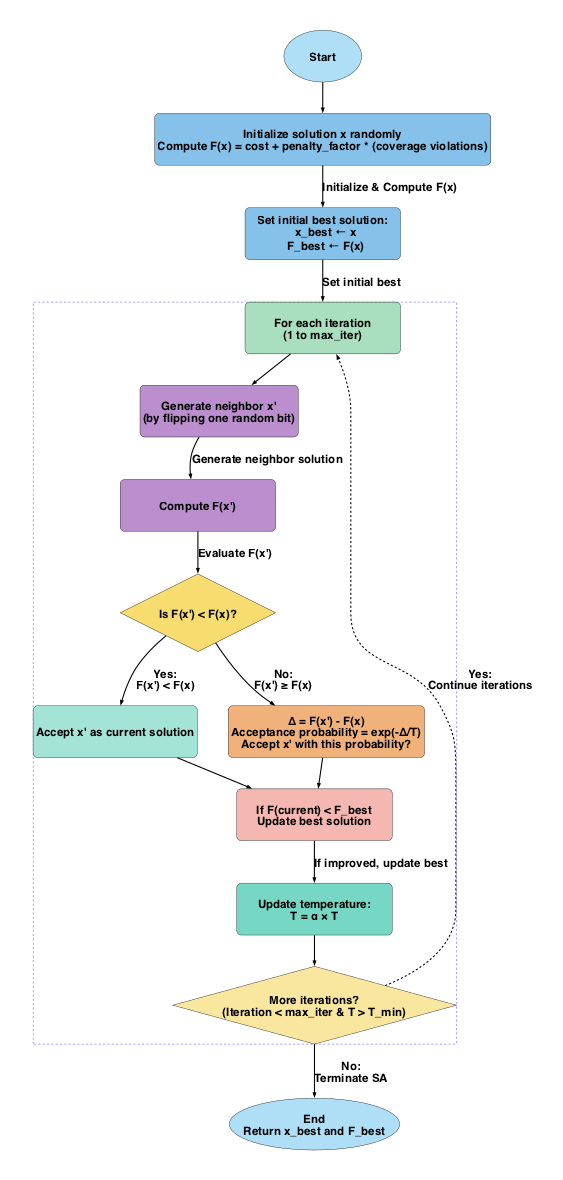
\includegraphics[width=0.60\textwidth]{simulated_annealing_flowchart.png}
  \caption{Flowchart of the Simulated Annealing Algorithm for the Set Partitioning Problem.}
  \label{fig:flowchart1}
\end{figure}

\newpage

\subsection{Standard Binary Genetic Algorithm (BGA)}
The Standard Binary Genetic Algorithm is a population-based technique that evolves a set of candidate solutions using selection, crossover, and mutation operators. It utilises tournament selection to choose parents, applies one-point crossover to combine their genetic material, and uses bit-flip mutation to introduce variability. A penalty function is employed to combine the cost of a solution with constraint violations, ensuring that feasibility is encouraged over generations. This method is well-suited for problems with discrete binary representations and offers robustness through its stochastic operations.

\subsubsection{Pseudocode}
The pseudocode below outlines the Standard Binary Genetic Algorithm for the SPP, detailing population initialization, tournament selection, crossover, mutation, and population update.
\begin{algorithm}[htbp]
  \caption{StandardBGA(popSize, cxRate, mutRate, maxGens, penaltyFactor, tournK)}
  \begin{algorithmic}[1]
    \State \(P \gets \text{RandomPopulation}(popSize)\) \Comment{Initialize population}
    \State \(\text{EvaluateFitness}(P,\,\text{penaltyFactor})\) \Comment{Evaluate fitness}
    \For{\(g = 1\) to maxGens}
      \State \(Q \gets \emptyset\) \Comment{New offspring}
      \While{\(|Q| < \text{popSize}\)}
        \State \(p_1 \gets \text{TournamentSelect}(P,\, tournamentK)\) \Comment{Select parent 1}
        \State \(p_2 \gets \text{TournamentSelect}(P,\, tournamentK)\) \Comment{Select parent 2}
        \If{\(\text{rand}() < cxRate\)}
          \State \((c_1, c_2) \gets \text{OnePointCrossover}(p_1, p_2)\) \Comment{Crossover}
        \Else
          \State \(c_1 \gets p_1,\; c_2 \gets p_2\) \Comment{Copy parents}
        \EndIf
        \State \(\text{Mutate}(c_1,\, mutRate)\) \Comment{Mutate child 1}
        \State \(\text{Mutate}(c_2,\, mutRate)\) \Comment{Mutate child 2}
        \State \(\text{EvaluateFitness}(\{c_1, c_2\},\, \text{penaltyFactor})\) \Comment{Evaluate offspring}
        \State \(Q \gets Q \cup \{c_1, c_2\}\) \Comment{Add offspring}
      \EndWhile
      \State \(P \gets Q\) \Comment{Update population}
    \EndFor
    \State \Return \(\text{BestSolution}(P)\) \Comment{Return best solution}
  \end{algorithmic}
  \end{algorithm}

\subsubsection{Flowchart}
The flowchart provides a visual overview of the Standard BGA’s iterative process, from offspring generation to re-ranking and best solution update.

\begin{figure}[htbp]
  \centering
  % Adjust the width as needed, e.g., 0.9\textwidth fills most of the page width
  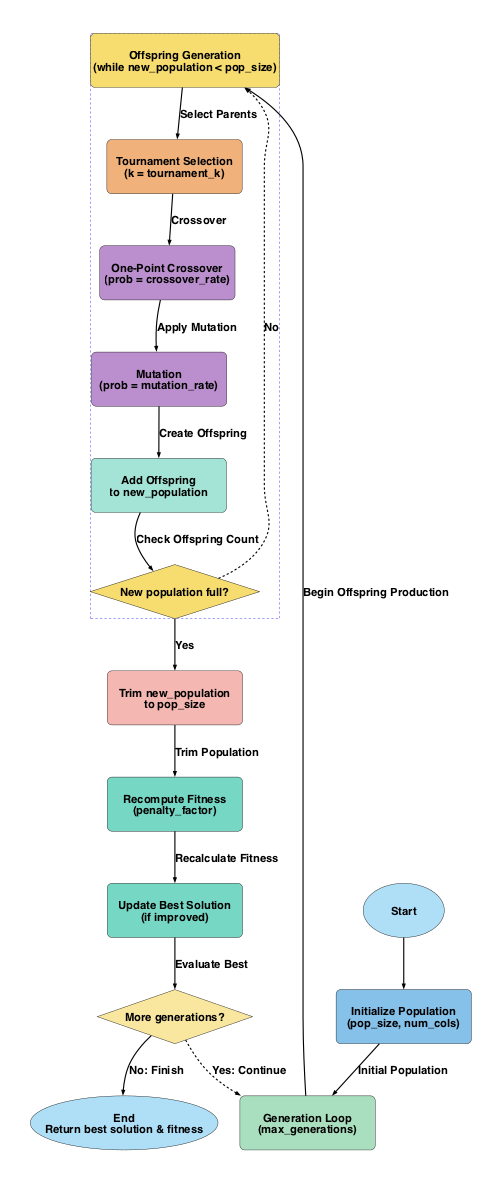
\includegraphics[width=0.55\textwidth]{standard_bga_flowchart.png}
  \caption{Flowchart of the Standard Binary Genetic Algorithm for the Set Partitioning Problem.}
  \label{fig:flowchart2}
\end{figure}

\newpage

\subsection{Improved Binary Genetic Algorithm (BGA)}
The Improved Binary Genetic Algorithm extends the standard BGA by integrating several problem-specific enhancements. It begins with a pseudo–random initialisation that aims to reduce over–coverage in the initial population. The algorithm then incorporates a stochastic ranking procedure that probabilistically balances cost and constraint violation, allowing for a more flexible handling of infeasible solutions. Adaptive mutation is employed to reintroduce promising genetic material, and a DROP/ADD heuristic improvement operator repairs infeasible solutions. These enhancements, inspired by Chu \& Beasley~\cite{ChuAndBeasley1998} and Runarsson \& Yao~\cite{RunarssonYao2000}, make the Improved BGA particularly robust for the SPP. Overall, this algorithm offers a more sophisticated search mechanism by blending global search operators with domain-specific repairs.

\subsubsection{Pseudocode}
The pseudocode below describes the Improved Binary Genetic Algorithm for the SPP, integrating pseudo–random initialization, stochastic ranking, adaptive mutation, and heuristic repair.
\begin{algorithm}[htbp]
  \caption{ImprovedBGA(popSize, maxGens, \(p_{\mathrm{stoch}}\), ...)}
  \begin{algorithmic}[1]
    \State \(P \gets \text{PseudoRandomInit}(popSize)\) \Comment{Initialize population}
    \State \(\text{EvaluateCostUnfitness}(P)\) \Comment{Evaluate individuals}
    \For{\(g = 1\) to maxGens}
      \State \(\text{StochasticRankSort}(P, p_{\mathrm{stoch}})\) \Comment{Rank population}
      \State \(O \gets \emptyset\) \Comment{Reset offspring}
      \While{\(|O| < popSize\)}
        \State \((p_1, p_2) \gets \text{SelectParents}(P)\) \Comment{Select parents}
        \State \((c_1, c_2) \gets \text{UniformCrossover}(p_1, p_2)\) \Comment{Crossover}
        \State \(\text{AdaptiveMutation}(c_1, P)\) \Comment{Mutate child 1}
        \State \(\text{AdaptiveMutation}(c_2, P)\) \Comment{Mutate child 2}
        \State \(\text{HeuristicImprove}(c_1)\) \Comment{Repair child 1}
        \State \(\text{HeuristicImprove}(c_2)\) \Comment{Repair child 2}
        \State \(\text{EvaluateCostUnfitness}(\{c_1, c_2\})\) \Comment{Evaluate offspring}
        \State \(O \gets O \cup \{c_1, c_2\}\) \Comment{Add offspring}
      \EndWhile
      \State \(C \gets P \cup O\) \Comment{Combine populations}
      \State \(\text{StochasticRankSort}(C, p_{\mathrm{stoch}})\) \Comment{Rank combined pop}
      \State \(P \gets \text{Top}(C, popSize)\) \Comment{Select top individuals}
    \EndFor
    \State \Return \(\text{BestFeasible}(P)\) \Comment{Return best feasible solution}
  \end{algorithmic}
  \end{algorithm}

\subsubsection{Flowchart}
The flowchart visually maps the Enhanced BGA’s process, clearly highlighting its advanced offspring production and repair mechanisms.
\begin{figure}[htbp]
  \centering
  % Adjust the width as needed, e.g., 0.9\textwidth fills most of the page width
  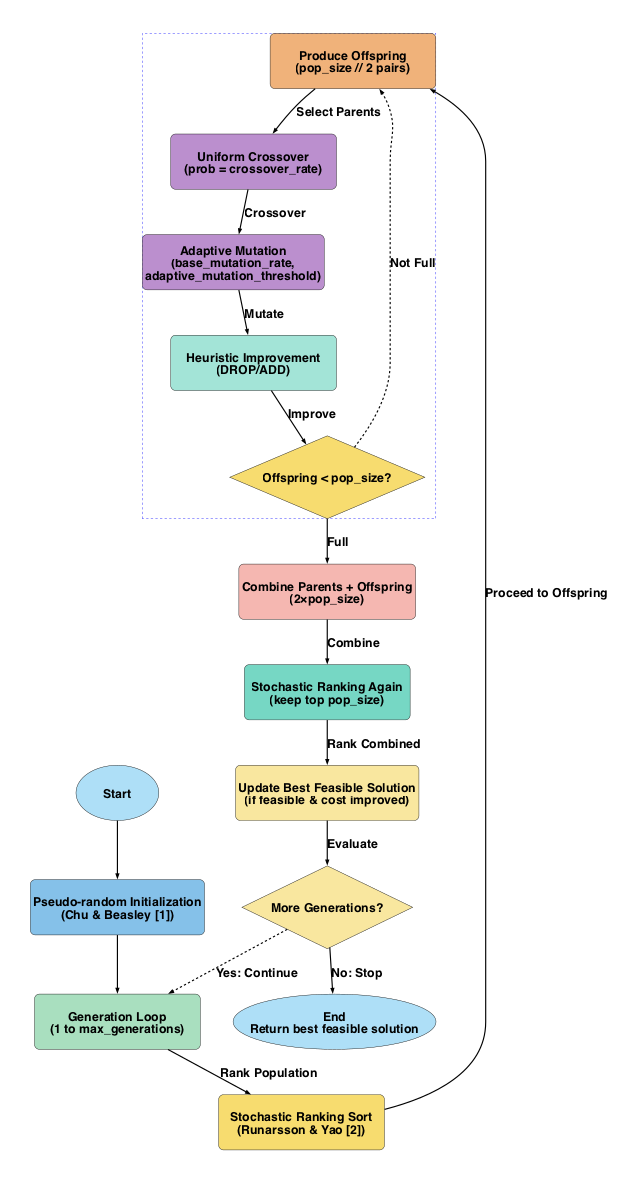
\includegraphics[width=0.70\textwidth]{improved_bga_flowchart.png}
  \caption{Flowchart of the Improved Binary Genetic Algorithm for the Set Partitioning Problem.}
  \label{fig:flowchart3}
\end{figure}

\newpage

\section{Benchmark Results}
\label{sec:results}

\newpage

\section{Discussion and Comparison}
\label{sec:discussion}

\newpage

\section{Ranking Replacement vs. Stochastic Ranking}
\label{sec:ranking}
Both methods aim to balance cost and constraint satisfaction in the SPP, yet they differ in approach. The \textbf{Ranking Replacement} method (Chu \& Beasley, 1998) partitions the population deterministically into four subgroups based on fitness (cost) and unfitness (constraint violation). A new solution replaces an individual from the first non-empty subgroup (starting with those worst in both criteria), thereby steadily improving the overall population. This approach offers a clear structure but can be rigid as the balance between cost and constraint violation may evolve during the search.

In contrast, the \textbf{Stochastic Ranking} method (Runarsson \& Yao, 2000) uses a bubble-sort-like procedure where adjacent solutions are compared probabilistically—if at least one solution is infeasible, they are compared by cost with a set probability \(P\) (typically less than 0.5) and by unfitness otherwise. This allows for a more adaptive balance, enabling the search to explore infeasible regions as bridges between isolated feasible areas without rigid subgroup thresholds.

In summary, while both methods share the goal of guiding the search toward feasible, high-quality solutions, Ranking Replacement enforces a strict hierarchical structure, whereas Stochastic Ranking offers a flexible, adaptive mechanism that reduces the need for extensive parameter tuning.
\section{Conclusion}
This report has presented three advanced algorithms for solving airline crew scheduling problems: Simulated Annealing, a Standard Binary Genetic Algorithm, and an Improved Binary Genetic Algorithm incorporating problem-specific enhancements. Detailed, moderately sized flowcharts and refined pseudocode have been provided to elucidate each method's internal workings. Benchmark results and an in-depth discussion will be appended once experiments are complete. Furthermore, a comparative discussion on constraint-handling—contrasting ranking replacement and stochastic ranking—has been included, underscoring the adaptive advantages of the latter.

\newpage

\begin{thebibliography}{9}
\bibitem{ChuAndBeasley1998}
  P.~C. Chu and J.~E. Beasley, 
  \emph{Constraint Handling in Genetic Algorithms: The Set Partitioning Problem},
  Journal of Heuristics, 11:323--357, 1998.

\bibitem{RunarssonYao2000}
  T.~P. Runarsson and X. Yao, 
  \emph{Stochastic Ranking for Constrained Evolutionary Optimisation},
  IEEE Transactions on Evolutionary Computation, 4(3):284--294, 2000.
\end{thebibliography}

\end{document}